\documentclass[12pt,a4paper]{article}

\usepackage[left=2cm,right=2cm,top=2cm,bottom=2cm]{geometry} % less blank area
\usepackage{amsmath,bm} % for math
\usepackage{array}   % for eqnarray
\usepackage{graphicx}
\usepackage{listings} % for code demonstration
\usepackage{color}    % for code highlight
\usepackage{fancyhdr} % for header and footnote
\usepackage{lastpage} % for calculating total pages
\usepackage{subfig} % for subfigure
\usepackage{tikz} % for drawing

\newcommand{\docTitle}{Practical Course -- Vision-based Navigation: Exercise \#1}
\newcommand{\docAuthor}{Min-An Chao (03681062)}
\newcommand{\docAuthorDept}{TUM MS Informatics}
\newcommand{\docAuthorEmail}{ga83fok@mytum.de}
\newcommand{\docDate}{22.04.2018}

\pagestyle{fancy}
\fancyhf{}
\lhead{\textit{\docTitle}}
\rhead{\textit{\docAuthor}}
\cfoot{\textit{- Page \thepage of \pageref{LastPage} -}}

\lstset{ language=c++,
         basicstyle=\ttfamily\footnotesize,
         keywordstyle=\color{blue}\ttfamily\footnotesize,
         commentstyle=\color{magenta}\ttfamily\footnotesize,
         morecomment=[l][\color{magenta}\footnotesize]{\#}
}

\setlength{\parindent}{0cm}
\setlength{\parskip}{0.5cm}


\begin{document}
    \title{\vspace{-1.75cm} \large \textsf{\textbf{\docTitle}}}
    \author{\normalsize \textsf{
        \textbf{\docAuthor} \hspace{6pt}\textbar\hspace{6pt}
        \docAuthorDept \hspace{6pt}\textbar\hspace{6pt}
        \docAuthorEmail}}
    \date{\small \textsf{\docDate}}
    \maketitle 
    \thispagestyle{fancy}
    \vspace{-0.5cm}
    \hrule

    \section{What is SLAM}
   
    \textsf{\textbf{Problem 1}}
    
    \textsf{\textbf{Problem 2}}
    
    \textsf{\textbf{Problem 3}}

    \section{Using \texttt{cmake} to manage SLAM projects written in C++}
    \textsf{\textbf{Task 1}}


    \textsf{\textbf{Task 2}}
    As shown in Fig.~\ref{fig:orbslam_snapshot},

    \begin{figure}[!h]
        \centering
        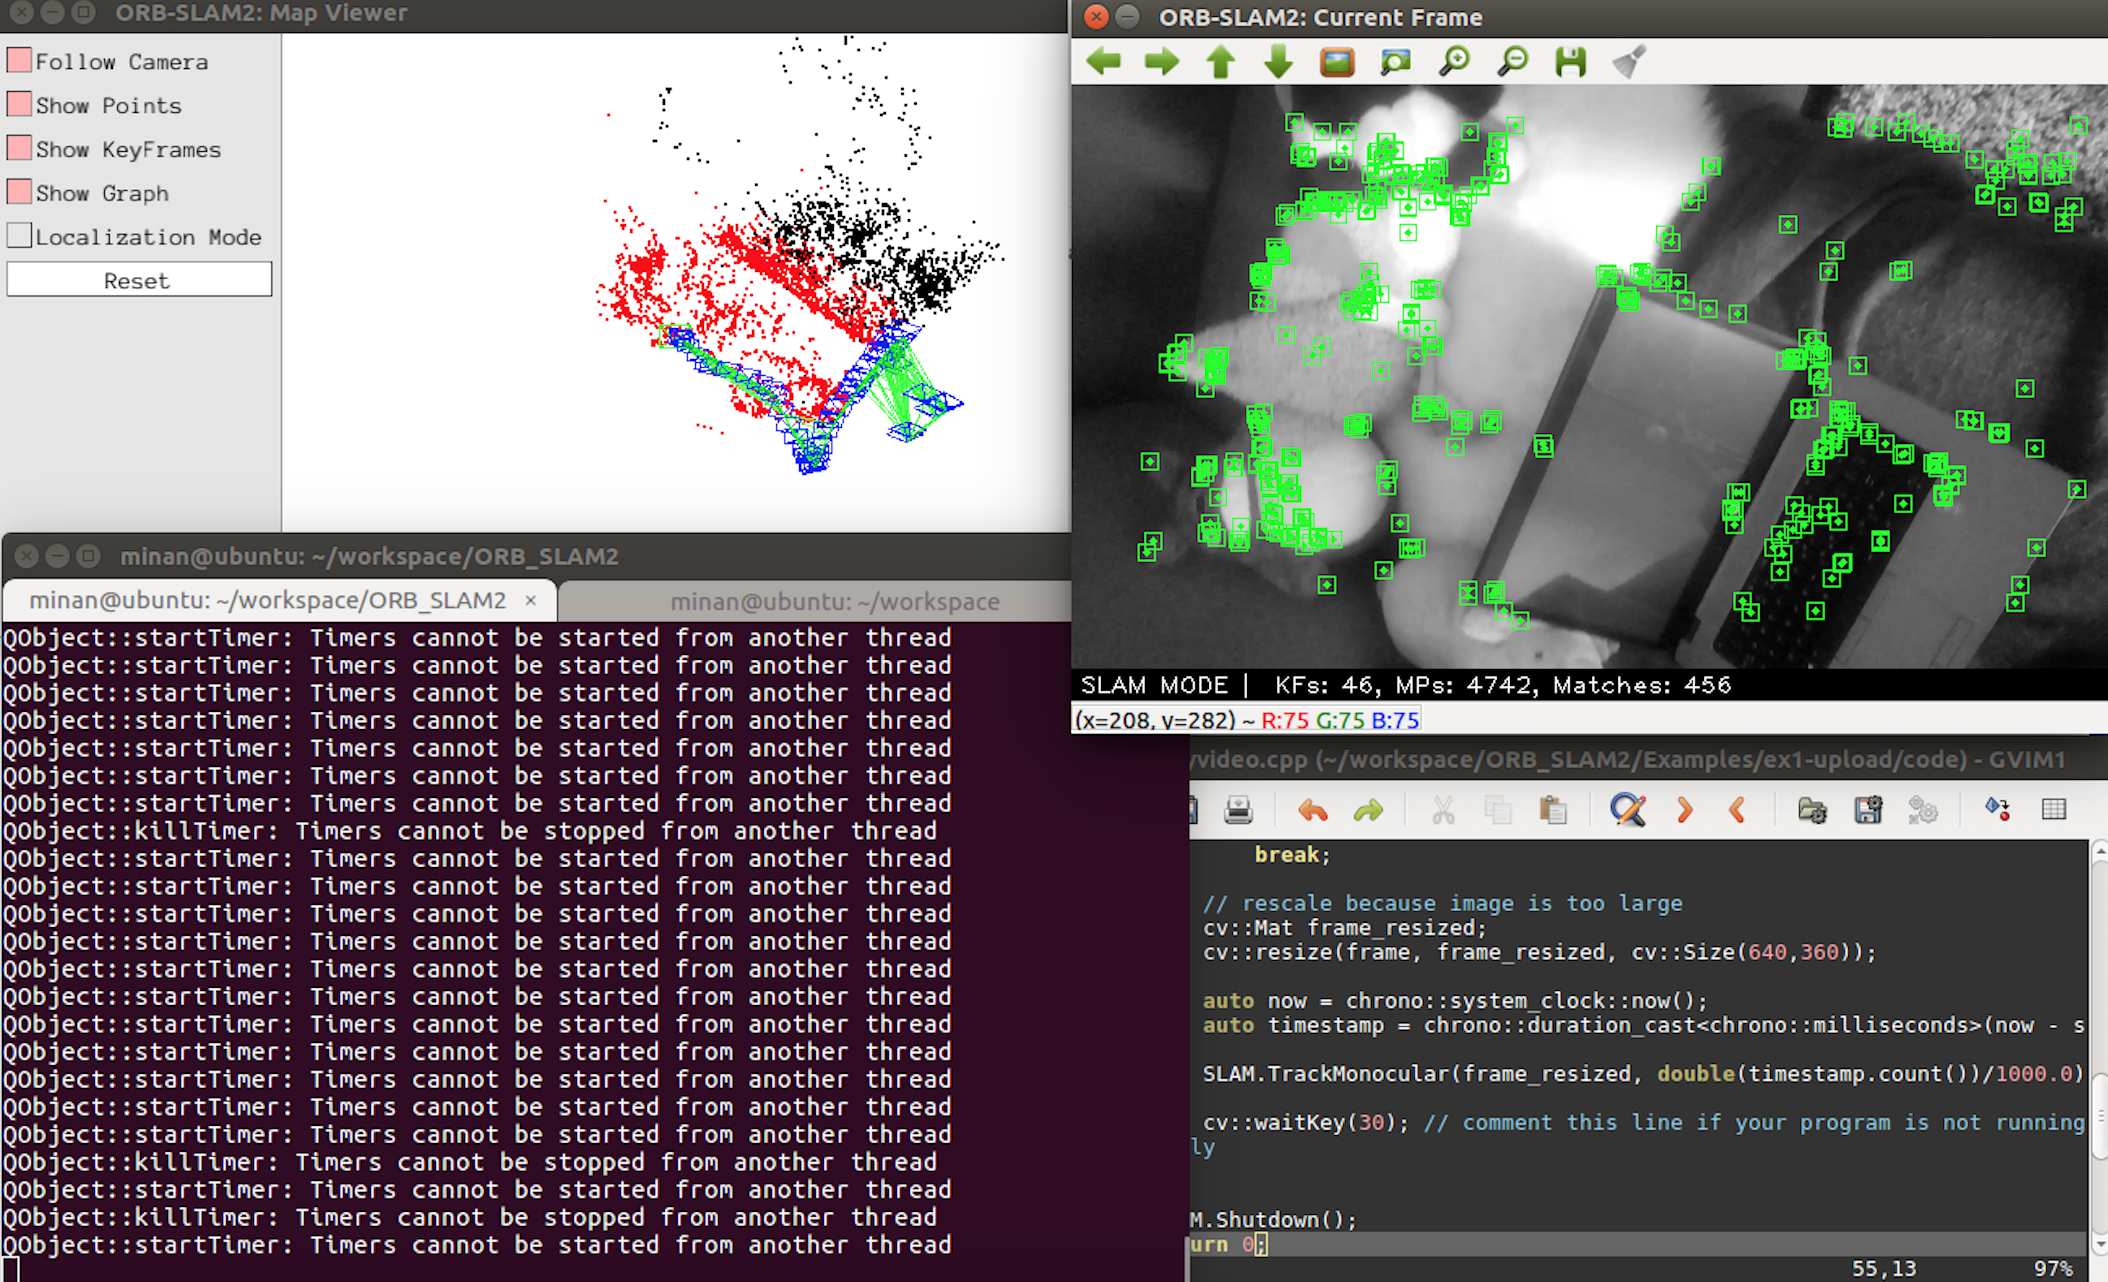
\includegraphics[height=6cm]{fig/orbslam_snapshot.png}
        \caption{Snapshot of \texttt{ORB-SLAM2} running on \texttt{mp4} video clip}
        \label{fig:orbslam_snapshot}
    \end{figure}
    
    \section{Using \texttt{Eigen} library to handle geometry computation}
    \textsf{\textbf{Task 1}}

    \textsf{\textbf{Task 2}}
    
    \textsf{\textbf{Task 3}}
    
    
\end{document}
